\documentclass[twoside]{book}

% Packages required by doxygen
\usepackage{fixltx2e}
\usepackage{calc}
\usepackage{doxygen}
\usepackage[export]{adjustbox} % also loads graphicx
\usepackage{graphicx}
\usepackage[utf8]{inputenc}
\usepackage{makeidx}
\usepackage{multicol}
\usepackage{multirow}
\PassOptionsToPackage{warn}{textcomp}
\usepackage{textcomp}
\usepackage[nointegrals]{wasysym}
\usepackage[table]{xcolor}

% Font selection
\usepackage[T1]{fontenc}
\usepackage[scaled=.90]{helvet}
\usepackage{courier}
\usepackage{amssymb}
\usepackage{sectsty}
\renewcommand{\familydefault}{\sfdefault}
\allsectionsfont{%
  \fontseries{bc}\selectfont%
  \color{darkgray}%
}
\renewcommand{\DoxyLabelFont}{%
  \fontseries{bc}\selectfont%
  \color{darkgray}%
}
\newcommand{\+}{\discretionary{\mbox{\scriptsize$\hookleftarrow$}}{}{}}

% Page & text layout
\usepackage{geometry}
\geometry{%
  a4paper,%
  top=2.5cm,%
  bottom=2.5cm,%
  left=2.5cm,%
  right=2.5cm%
}
\tolerance=750
\hfuzz=15pt
\hbadness=750
\setlength{\emergencystretch}{15pt}
\setlength{\parindent}{0cm}
\setlength{\parskip}{3ex plus 2ex minus 2ex}
\makeatletter
\renewcommand{\paragraph}{%
  \@startsection{paragraph}{4}{0ex}{-1.0ex}{1.0ex}{%
    \normalfont\normalsize\bfseries\SS@parafont%
  }%
}
\renewcommand{\subparagraph}{%
  \@startsection{subparagraph}{5}{0ex}{-1.0ex}{1.0ex}{%
    \normalfont\normalsize\bfseries\SS@subparafont%
  }%
}
\makeatother

% Headers & footers
\usepackage{fancyhdr}
\pagestyle{fancyplain}
\fancyhead[LE]{\fancyplain{}{\bfseries\thepage}}
\fancyhead[CE]{\fancyplain{}{}}
\fancyhead[RE]{\fancyplain{}{\bfseries\leftmark}}
\fancyhead[LO]{\fancyplain{}{\bfseries\rightmark}}
\fancyhead[CO]{\fancyplain{}{}}
\fancyhead[RO]{\fancyplain{}{\bfseries\thepage}}
\fancyfoot[LE]{\fancyplain{}{}}
\fancyfoot[CE]{\fancyplain{}{}}
\fancyfoot[RE]{\fancyplain{}{\bfseries\scriptsize Generated by Doxygen }}
\fancyfoot[LO]{\fancyplain{}{\bfseries\scriptsize Generated by Doxygen }}
\fancyfoot[CO]{\fancyplain{}{}}
\fancyfoot[RO]{\fancyplain{}{}}
\renewcommand{\footrulewidth}{0.4pt}
\renewcommand{\chaptermark}[1]{%
  \markboth{#1}{}%
}
\renewcommand{\sectionmark}[1]{%
  \markright{\thesection\ #1}%
}

% Indices & bibliography
\usepackage{natbib}
\usepackage[titles]{tocloft}
\setcounter{tocdepth}{3}
\setcounter{secnumdepth}{5}
\makeindex

% Hyperlinks (required, but should be loaded last)
\usepackage{ifpdf}
\ifpdf
  \usepackage[pdftex,pagebackref=true]{hyperref}
\else
  \usepackage[ps2pdf,pagebackref=true]{hyperref}
\fi
\hypersetup{%
  colorlinks=true,%
  linkcolor=blue,%
  citecolor=blue,%
  unicode%
}

% Custom commands
\newcommand{\clearemptydoublepage}{%
  \newpage{\pagestyle{empty}\cleardoublepage}%
}

\usepackage{caption}
\captionsetup{labelsep=space,justification=centering,font={bf},singlelinecheck=off,skip=4pt,position=top}

%===== C O N T E N T S =====

\begin{document}

% Titlepage & ToC
\hypersetup{pageanchor=false,
             bookmarksnumbered=true,
             pdfencoding=unicode
            }
\pagenumbering{alph}
\begin{titlepage}
\vspace*{7cm}
\begin{center}%
{\Large Solid Transformations }\\
\vspace*{1cm}
{\large Generated by Doxygen 1.8.13}\\
\end{center}
\end{titlepage}
\clearemptydoublepage
\pagenumbering{roman}
\tableofcontents
\clearemptydoublepage
\pagenumbering{arabic}
\hypersetup{pageanchor=true}

%--- Begin generated contents ---
\chapter{Class Index}
\section{Class List}
Here are the classes, structs, unions and interfaces with brief descriptions\+:\begin{DoxyCompactList}
\item\contentsline{section}{\hyperlink{classtransformations}{transformations} }{\pageref{classtransformations}}{}
\end{DoxyCompactList}

\chapter{File Index}
\section{File List}
Here is a list of all documented files with brief descriptions\+:\begin{DoxyCompactList}
\item\contentsline{section}{include/solid\+\_\+trans/\hyperlink{Transformations_8h}{Transformations.\+h} \\*Defines \hyperlink{classTransformations}{Transformations} class for performing rigid-\/body transformations }{\pageref{Transformations_8h}}{}
\item\contentsline{section}{src/\hyperlink{Transformations_8cpp}{Transformations.\+cpp} \\*Implements \hyperlink{Transformations_8h}{Transformations.\+h} }{\pageref{Transformations_8cpp}}{}
\end{DoxyCompactList}

\chapter{Class Documentation}
\hypertarget{classTransformations}{}\section{Transformations Class Reference}
\label{classTransformations}\index{Transformations@{Transformations}}


Returns 4x4 Trasnformation Matrix for basic rigid-\/body transformations.  




{\ttfamily \#include $<$Transformations.\+h$>$}

\subsection*{Public Member Functions}
\begin{DoxyCompactItemize}
\item 
Eigen\+::\+Matrix4d \hyperlink{classTransformations_a986ab195864427749bcba507a2d5fe58}{reflectX} ()
\begin{DoxyCompactList}\small\item\em Returns Transformation Matrix for reflecting about YZ plane. \end{DoxyCompactList}\item 
Eigen\+::\+Matrix4d \hyperlink{classTransformations_a3ff59b80990ec879ed6d534dc620cee3}{reflectY} ()
\begin{DoxyCompactList}\small\item\em Returns Transformation Matrix for reflecting about XZ plane. \end{DoxyCompactList}\item 
Eigen\+::\+Matrix4d \hyperlink{classTransformations_afa74f1e98c9b69e368442c011d8cd046}{reflectZ} ()
\begin{DoxyCompactList}\small\item\em Returns Transformation Matrix for reflecting about XY plane. \end{DoxyCompactList}\item 
Eigen\+::\+Matrix4d \hyperlink{classTransformations_a9d470736a0a55415259c9eea0bf8a2e0}{rotate} (Eigen\+::\+Vector3f, double)
\begin{DoxyCompactList}\small\item\em Returns Transformation Matrix to rotate by \textquotesingle{}angle\textquotesingle{} angles about \textquotesingle{}axis\textquotesingle{} axis. \end{DoxyCompactList}\item 
Eigen\+::\+Matrix4d \hyperlink{classTransformations_a4c54165181c5d5ec5bb7db9e3176c4a7}{rotateX} (double)
\begin{DoxyCompactList}\small\item\em Returns Transformation Matrix for rotating about X-\/axis by \textquotesingle{}angle\textquotesingle{} angles. \end{DoxyCompactList}\item 
Eigen\+::\+Matrix4d \hyperlink{classTransformations_aa4a1b79a607ba97fa839c7f247ebc4df}{rotateY} (double)
\begin{DoxyCompactList}\small\item\em Returns Transformation Matrix for rotating about Y-\/axis by \textquotesingle{}angle\textquotesingle{} angles. \end{DoxyCompactList}\item 
Eigen\+::\+Matrix4d \hyperlink{classTransformations_af700b3a14795f2483e73dac667138907}{rotateZ} (double)
\begin{DoxyCompactList}\small\item\em Returns Transformation Matrix for rotating about Z-\/axis by \textquotesingle{}angle\textquotesingle{} angles. \end{DoxyCompactList}\item 
Eigen\+::\+Matrix4d \hyperlink{classTransformations_a7b7212f21b4e71ea50526e8359d74929}{translate} (Eigen\+::\+Vector3d)
\begin{DoxyCompactList}\small\item\em Returns Transformation Matrix for translation. \end{DoxyCompactList}\item 
Eigen\+::\+Matrix4d \hyperlink{classTransformations_a0948151585af910e7bd2c6734ecf9d5b}{scale\+All} (const double)
\begin{DoxyCompactList}\small\item\em Returns Transformation Matrix for Scaling of all dimensions. \end{DoxyCompactList}\item 
Eigen\+::\+Matrix4d \hyperlink{classTransformations_a43c9ba3fcb9d8fb440f3a686b8a99434}{scale} (const double, const double, const double)
\begin{DoxyCompactList}\small\item\em Returns Transformation Matrix for Scaling of dimensions along principal axes. \end{DoxyCompactList}\item 
\mbox{\Hypertarget{classTransformations_a3dddecc6c02addaaa804e0c3ebb8163f}\label{classTransformations_a3dddecc6c02addaaa804e0c3ebb8163f}} 
\hyperlink{classTransformations_a3dddecc6c02addaaa804e0c3ebb8163f}{Transformations} ()
\begin{DoxyCompactList}\small\item\em Construct a new \hyperlink{classTransformations}{Transformations}\+:\+: \hyperlink{classTransformations}{Transformations} object. \end{DoxyCompactList}\end{DoxyCompactItemize}


\subsection{Detailed Description}
Returns 4x4 Trasnformation Matrix for basic rigid-\/body transformations. 

\subsection{Member Function Documentation}
\mbox{\Hypertarget{classTransformations_a986ab195864427749bcba507a2d5fe58}\label{classTransformations_a986ab195864427749bcba507a2d5fe58}} 
\index{Transformations@{Transformations}!reflectX@{reflectX}}
\index{reflectX@{reflectX}!Transformations@{Transformations}}
\subsubsection{\texorpdfstring{reflect\+X()}{reflectX()}}
{\footnotesize\ttfamily Eigen\+::\+Matrix4d Transformations\+::reflectX (\begin{DoxyParamCaption}{ }\end{DoxyParamCaption})}



Returns Transformation Matrix for reflecting about YZ plane. 

\begin{DoxyReturn}{Returns}
Eigen\+::\+Matrix4d Required 4x4 Transformation Matrix. 
\end{DoxyReturn}
\mbox{\Hypertarget{classTransformations_a3ff59b80990ec879ed6d534dc620cee3}\label{classTransformations_a3ff59b80990ec879ed6d534dc620cee3}} 
\index{Transformations@{Transformations}!reflectY@{reflectY}}
\index{reflectY@{reflectY}!Transformations@{Transformations}}
\subsubsection{\texorpdfstring{reflect\+Y()}{reflectY()}}
{\footnotesize\ttfamily Eigen\+::\+Matrix4d Transformations\+::reflectY (\begin{DoxyParamCaption}{ }\end{DoxyParamCaption})}



Returns Transformation Matrix for reflecting about XZ plane. 

\begin{DoxyReturn}{Returns}
Eigen\+::\+Matrix4d Required 4x4 Transformation Matrix. 
\end{DoxyReturn}
\mbox{\Hypertarget{classTransformations_afa74f1e98c9b69e368442c011d8cd046}\label{classTransformations_afa74f1e98c9b69e368442c011d8cd046}} 
\index{Transformations@{Transformations}!reflectZ@{reflectZ}}
\index{reflectZ@{reflectZ}!Transformations@{Transformations}}
\subsubsection{\texorpdfstring{reflect\+Z()}{reflectZ()}}
{\footnotesize\ttfamily Eigen\+::\+Matrix4d Transformations\+::reflectZ (\begin{DoxyParamCaption}{ }\end{DoxyParamCaption})}



Returns Transformation Matrix for reflecting about XY plane. 

\begin{DoxyReturn}{Returns}
Eigen\+::\+Matrix4d Required 4x4 Transformation Matrix. 
\end{DoxyReturn}
\mbox{\Hypertarget{classTransformations_a9d470736a0a55415259c9eea0bf8a2e0}\label{classTransformations_a9d470736a0a55415259c9eea0bf8a2e0}} 
\index{Transformations@{Transformations}!rotate@{rotate}}
\index{rotate@{rotate}!Transformations@{Transformations}}
\subsubsection{\texorpdfstring{rotate()}{rotate()}}
{\footnotesize\ttfamily Eigen\+::\+Matrix4d Transformations\+::rotate (\begin{DoxyParamCaption}\item[{Eigen\+::\+Vector3f}]{axis,  }\item[{double}]{angle }\end{DoxyParamCaption})}



Returns Transformation Matrix to rotate by \textquotesingle{}angle\textquotesingle{} angles about \textquotesingle{}axis\textquotesingle{} axis. 


\begin{DoxyParams}{Parameters}
{\em axis} & 3D Vector denoting the rotation axis. \\
\hline
{\em angle} & in radians. \\
\hline
\end{DoxyParams}
\begin{DoxyReturn}{Returns}
Eigen\+::\+Matrix4d The required 4x4 Transformation Matrix. 
\end{DoxyReturn}
\mbox{\Hypertarget{classTransformations_a4c54165181c5d5ec5bb7db9e3176c4a7}\label{classTransformations_a4c54165181c5d5ec5bb7db9e3176c4a7}} 
\index{Transformations@{Transformations}!rotateX@{rotateX}}
\index{rotateX@{rotateX}!Transformations@{Transformations}}
\subsubsection{\texorpdfstring{rotate\+X()}{rotateX()}}
{\footnotesize\ttfamily Eigen\+::\+Matrix4d Transformations\+::rotateX (\begin{DoxyParamCaption}\item[{double}]{angle }\end{DoxyParamCaption})}



Returns Transformation Matrix for rotating about X-\/axis by \textquotesingle{}angle\textquotesingle{} angles. 


\begin{DoxyParams}{Parameters}
{\em angle} & in radians. \\
\hline
\end{DoxyParams}
\begin{DoxyReturn}{Returns}
Eigen\+::\+Matrix4d Required 4x4 Transformation Matrix. 
\end{DoxyReturn}
\mbox{\Hypertarget{classTransformations_aa4a1b79a607ba97fa839c7f247ebc4df}\label{classTransformations_aa4a1b79a607ba97fa839c7f247ebc4df}} 
\index{Transformations@{Transformations}!rotateY@{rotateY}}
\index{rotateY@{rotateY}!Transformations@{Transformations}}
\subsubsection{\texorpdfstring{rotate\+Y()}{rotateY()}}
{\footnotesize\ttfamily Eigen\+::\+Matrix4d Transformations\+::rotateY (\begin{DoxyParamCaption}\item[{double}]{angle }\end{DoxyParamCaption})}



Returns Transformation Matrix for rotating about Y-\/axis by \textquotesingle{}angle\textquotesingle{} angles. 


\begin{DoxyParams}{Parameters}
{\em angle} & in radians. \\
\hline
\end{DoxyParams}
\begin{DoxyReturn}{Returns}
Eigen\+::\+Matrix4d Required 4x4 Transformation Matrix. 
\end{DoxyReturn}
\mbox{\Hypertarget{classTransformations_af700b3a14795f2483e73dac667138907}\label{classTransformations_af700b3a14795f2483e73dac667138907}} 
\index{Transformations@{Transformations}!rotateZ@{rotateZ}}
\index{rotateZ@{rotateZ}!Transformations@{Transformations}}
\subsubsection{\texorpdfstring{rotate\+Z()}{rotateZ()}}
{\footnotesize\ttfamily Eigen\+::\+Matrix4d Transformations\+::rotateZ (\begin{DoxyParamCaption}\item[{double}]{angle }\end{DoxyParamCaption})}



Returns Transformation Matrix for rotating about Z-\/axis by \textquotesingle{}angle\textquotesingle{} angles. 


\begin{DoxyParams}{Parameters}
{\em angle} & in radians. \\
\hline
\end{DoxyParams}
\begin{DoxyReturn}{Returns}
Eigen\+::\+Matrix4d Required 4x4 Transformation Matrix. 
\end{DoxyReturn}
\mbox{\Hypertarget{classTransformations_a43c9ba3fcb9d8fb440f3a686b8a99434}\label{classTransformations_a43c9ba3fcb9d8fb440f3a686b8a99434}} 
\index{Transformations@{Transformations}!scale@{scale}}
\index{scale@{scale}!Transformations@{Transformations}}
\subsubsection{\texorpdfstring{scale()}{scale()}}
{\footnotesize\ttfamily Eigen\+::\+Matrix4d Transformations\+::scale (\begin{DoxyParamCaption}\item[{const double}]{factorX,  }\item[{const double}]{factorY,  }\item[{const double}]{factorZ }\end{DoxyParamCaption})}



Returns Transformation Matrix for Scaling of dimensions along principal axes. 


\begin{DoxyParams}{Parameters}
{\em factorX} & x-\/scaling \\
\hline
{\em factorY} & y-\/scaling \\
\hline
{\em factorZ} & z-\/scaling \\
\hline
\end{DoxyParams}
\begin{DoxyReturn}{Returns}
Eigen\+::\+Matrix4d Required 4x4 Transformation Matrix. 
\end{DoxyReturn}
\mbox{\Hypertarget{classTransformations_a0948151585af910e7bd2c6734ecf9d5b}\label{classTransformations_a0948151585af910e7bd2c6734ecf9d5b}} 
\index{Transformations@{Transformations}!scale\+All@{scale\+All}}
\index{scale\+All@{scale\+All}!Transformations@{Transformations}}
\subsubsection{\texorpdfstring{scale\+All()}{scaleAll()}}
{\footnotesize\ttfamily Eigen\+::\+Matrix4d Transformations\+::scale\+All (\begin{DoxyParamCaption}\item[{const double}]{factor }\end{DoxyParamCaption})}



Returns Transformation Matrix for Scaling of all dimensions. 


\begin{DoxyParams}{Parameters}
{\em factor} & \\
\hline
\end{DoxyParams}
\begin{DoxyReturn}{Returns}
Eigen\+::\+Matrix4d Required 4x4 Transformation Matrix. 
\end{DoxyReturn}
\mbox{\Hypertarget{classTransformations_a7b7212f21b4e71ea50526e8359d74929}\label{classTransformations_a7b7212f21b4e71ea50526e8359d74929}} 
\index{Transformations@{Transformations}!translate@{translate}}
\index{translate@{translate}!Transformations@{Transformations}}
\subsubsection{\texorpdfstring{translate()}{translate()}}
{\footnotesize\ttfamily Eigen\+::\+Matrix4d Transformations\+::translate (\begin{DoxyParamCaption}\item[{Eigen\+::\+Vector3d}]{displacement }\end{DoxyParamCaption})}



Returns Transformation Matrix for translation. 


\begin{DoxyParams}{Parameters}
{\em displacement} & in metres \\
\hline
\end{DoxyParams}
\begin{DoxyReturn}{Returns}
Eigen\+::\+Matrix4d Required 4x4 Transformation Matrix. 
\end{DoxyReturn}


The documentation for this class was generated from the following files\+:\begin{DoxyCompactItemize}
\item 
include/solid\+\_\+trans/\hyperlink{Transformations_8h}{Transformations.\+h}\item 
src/\hyperlink{Transformations_8cpp}{Transformations.\+cpp}\end{DoxyCompactItemize}

\chapter{File Documentation}
\hypertarget{Transformations_8cpp}{}\section{src/\+Transformations.cpp File Reference}
\label{Transformations_8cpp}\index{src/\+Transformations.\+cpp@{src/\+Transformations.\+cpp}}


implements \hyperlink{Transformations_8h}{Transformations.\+h}  


{\ttfamily \#include $<$solid\+\_\+trans/\+Transformations.\+h$>$}\newline
Include dependency graph for Transformations.\+cpp\+:\nopagebreak
\begin{figure}[H]
\begin{center}
\leavevmode
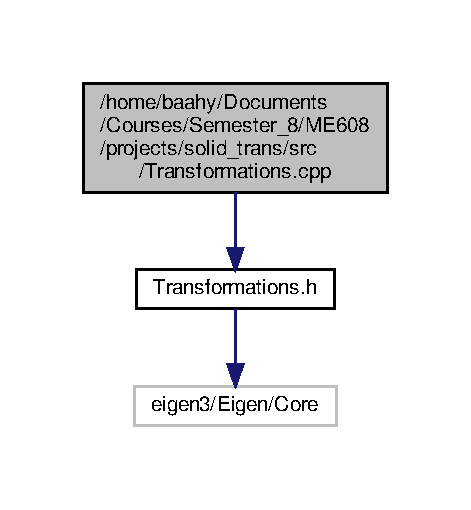
\includegraphics[width=226pt]{Transformations_8cpp__incl}
\end{center}
\end{figure}


\subsection{Detailed Description}
implements \hyperlink{Transformations_8h}{Transformations.\+h} 

\begin{DoxyAuthor}{Author}
Abhay Pratap Singh (\href{mailto:you@domain.com}{\tt you@domain.\+com}) 
\end{DoxyAuthor}
\begin{DoxyVersion}{Version}
0.\+1 
\end{DoxyVersion}
\begin{DoxyDate}{Date}
2020-\/03-\/26
\end{DoxyDate}
\begin{DoxyCopyright}{Copyright}
Copyright (c) 2020 
\end{DoxyCopyright}

%--- End generated contents ---

% Index
\backmatter
\newpage
\phantomsection
\clearemptydoublepage
\addcontentsline{toc}{chapter}{Index}
\printindex

\end{document}
